%!TEX root = ../dokumentation.tex

\chapter{Implementierung}
In diesem Kapitel geht es um die Implementierung des automatischen und manuellen Modus.

\section{Automatik Modus}
Im Modus Automatik wird die im folgenden Beschriebene Logik ausgeführt. Der Beweiser überführt dabei sogenannte Sequenten. Ein Sequent enthält alle Formeln auf der Wahr bzw. auf der Falsch Seite sowie einige weitere Mengen.

\subsection{Aussagenlogik}
Für die Aussagenlogik ist der Sequent S ein Sechstupel (T, F, $\Gamma$, $\Pi$, $\Theta$, $\Psi$). Die Mengen sind wie folgt definiert:
\begin{description}
\item \textbf{T}: Die Menge der Formeln auf der Wahr-Seite des Tableau.

\item \textbf{F}: Die Menge der Formeln auf der Falsch-Seite des Tableau.

\item \textbf{$\Gamma$}: Die Menge der Formeln die in vorherigen Ableitungsschritten abgeleitet wurden und dabei auf der Wahr-Seite standen.

\item \textbf{$\Pi$}: Die Menge der Formeln die in vorherigen Ableitungsschritten abgeleitet wurden und dabei auf der Falsch-Seite standen.

\item \textbf{$\Theta$}: Die Menge der atomaren Aussagen auf der Wahr-Seite.

\item \textbf{$\Psi$}: Die Menge der atomaren Aussagen auf der Falsch-Seite.
\end{description}

Der Beweiser muss nun im Automatik Modus eine Ableitung von S zu S' durchführen bis gilt $\exists\alpha$ ($\alpha\in\Theta\wedge\alpha\in\Psi$) $\vee\neg\exists\alpha$ ($\alpha\in$ T)$\wedge\neg\exists\alpha$ ($\alpha\in$ F). Ist eine Ableitung verzweigend, so wird von S zu S$_{1}$' und S$_{2}$' abgeleitet. Die Ableitungsregeln von S zu S' werden im folgenden definiert.

\subsubsection{Atomare Aussage}
Wenn $\alpha\in\textrm{T}$ dann folgt S'=($\textrm{T}\setminus\lbrace\alpha\rbrace$, F, $\Gamma\cup\lbrace\alpha\rbrace$, $\Pi$, $\Theta\cup\lbrace\alpha\rbrace$, $\Psi$).\\
Wenn $\alpha\in\textrm{F}$ dann folgt S'=(T, $\textrm{F}\setminus\lbrace\alpha\rbrace$, $\Gamma$, $\Pi\cup\lbrace\alpha\rbrace$, $\Theta$, $\Psi\cup\lbrace\alpha\rbrace$).

\subsubsection{Negation}
Wenn $\neg\alpha\in\textrm{T}$ dann folgt S'=($\textrm{T}\setminus\lbrace\neg\alpha\rbrace$, $\textrm{F}\cup\lbrace\alpha\rbrace$, $\Gamma\cup\lbrace\neg\alpha\rbrace$, $\Pi$, $\Theta$, $\Psi$).\\
Wenn $\neg\alpha\in\textrm{F}$ dann folgt S'=($\textrm{T}\cup\lbrace\alpha\rbrace$, $\textrm{F}\setminus\lbrace\neg\alpha\rbrace$, $\Gamma$, $\Pi\cup\lbrace\neg\alpha\rbrace$, $\Theta$, $\Psi$).

\subsubsection{Konjunktion}
Wenn $\alpha\wedge\beta\in\textrm{T}$ dann folgt S'=($(\textrm{T}\cup\lbrace\alpha,\beta\rbrace)\setminus\lbrace\alpha\wedge\beta\rbrace$, F, $\Gamma\cup\lbrace\alpha\wedge\beta\rbrace$, $\Pi$, $\Theta$, $\Psi$).\\
Wenn $\alpha\wedge\beta\in\textrm{F}$ dann folgt S$_{1}$'=($\textrm{T}\setminus\lbrace\alpha\wedge\beta\rbrace$, $\textrm{F}\cup\lbrace\alpha\rbrace$, $\Gamma$, $\Pi\cup\lbrace\alpha\wedge\beta\rbrace$, $\Theta$, $\Psi$) und S$_{2}$'=($\textrm{T}\setminus\lbrace\alpha\wedge\beta\rbrace$, $\textrm{F}\cup\lbrace\beta\rbrace$, $\Gamma$, $\Pi\cup\lbrace\alpha\wedge\beta\rbrace$, $\Theta$, $\Psi$).

\subsubsection{Disjunktion}
Wenn $\alpha\vee\beta\in\textrm{T}$ dann folgt S$_{1}$'=($(\textrm{T}\cup\lbrace\alpha\rbrace)\setminus\lbrace\alpha\vee\beta\rbrace$, F, $\Gamma\cup\lbrace\alpha\vee\beta\rbrace$, $\Pi$, $\Theta$, $\Psi$) und S$_{2}$'=($(\textrm{T}\cup\lbrace\beta\rbrace)\setminus\lbrace\alpha\vee\beta\rbrace$, F, $\Gamma\cup\lbrace\alpha\vee\beta\rbrace$, $\Pi$, $\Theta$, $\Psi$).\\
Wenn $\alpha\vee\beta\in\textrm{F}$ dann folgt S'=(T, $(\textrm{F}\cup\lbrace\alpha,\beta\rbrace)\setminus\lbrace\alpha\vee\beta\rbrace$, $\Gamma$, $\Pi\cup\lbrace\alpha\vee\beta\rbrace$, $\Theta$, $\Psi$).

\subsubsection{Implikation}
Wenn $\alpha\rightarrow\beta\in\textrm{T}$ dann folgt S$_{1}$'=($(\textrm{T}\cup\lbrace\alpha\rbrace)\setminus\lbrace\alpha\rightarrow\beta\rbrace$, F, $\Gamma\cup\lbrace\alpha\rightarrow\beta\rbrace$, $\Pi$, $\Theta$, $\Psi$) und S$_{2}$'=($\textrm{T}\setminus\lbrace\alpha\rightarrow\beta\rbrace$, $\textrm{F}\cup\lbrace\beta\rbrace$, $\Gamma\cup\lbrace\alpha\rightarrow\beta\rbrace$, $\Pi$, $\Theta$, $\Psi$).\\
Wenn $\alpha\rightarrow\beta\in\textrm{F}$ dann folgt S'=($\textrm{T}\cup\lbrace\alpha\rbrace$, $(\textrm{F}\cup\lbrace\beta\rbrace)\setminus\lbrace\alpha\rightarrow\beta\rbrace$, $\Gamma$, $\Pi\cup\lbrace\alpha\rightarrow\beta\rbrace$, $\Theta$, $\Psi$).

\subsubsection{Äquivalenz}
Wenn $\alpha\leftrightarrow\beta\in\textrm{T}$ dann folgt S$_{1}$'=($(\textrm{T}\cup\lbrace\alpha,\beta\rbrace)\setminus\lbrace\alpha\leftrightarrow\beta\rbrace$, F, $\Gamma\cup\lbrace\alpha\leftrightarrow\beta\rbrace$, $\Pi$, $\Theta$, $\Psi$) und S$_{2}$'=($\textrm{T}\setminus\lbrace\alpha\leftrightarrow\beta\rbrace$, $\textrm{F}\cup\lbrace\alpha,\beta\rbrace$, $\Gamma\cup\lbrace\alpha\leftrightarrow\beta\rbrace$, $\Pi$, $\Theta$, $\Psi$).\\
Wenn $\alpha\leftrightarrow\beta\in\textrm{F}$ dann folgt S$_{1}$'=($\textrm{T}\cup\lbrace\alpha\rbrace$, $(\textrm{F}\cup\lbrace\beta\rbrace)\setminus\lbrace\alpha\leftrightarrow\beta\rbrace$, $\Gamma$, $\Pi\cup\lbrace\alpha\leftrightarrow\beta\rbrace$, $\Theta$, $\Psi$) und S$_{2}$'=($\textrm{T}\cup\lbrace\beta\rbrace$, $(\textrm{F}\cup\lbrace\alpha\rbrace)\setminus\lbrace\alpha\leftrightarrow\beta\rbrace$, $\Gamma$, $\Pi\cup\lbrace\alpha\leftrightarrow\beta\rbrace$, $\Theta$, $\Psi$).

\subsubsection{Umsetzung}
Die definierten Ableitungsregeln, werden mit dem Visitor Pattern abgearbeitet. \cite{gof_design_patterns} Das zugehörige Klassendiagramm ist in \autoref{fig:class_diag_tableau_prover} dargestellt.

\begin{figure}[h]
\begin{center}
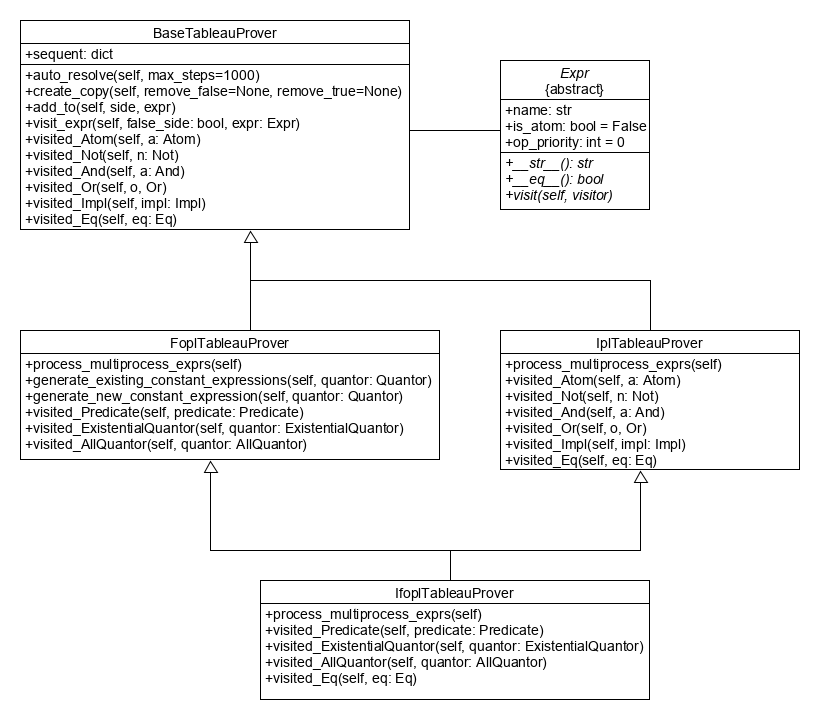
\includegraphics[scale=0.55]{images/class_diag_tableau_prover.png}
\caption{Klassendiagram des Tableau Beweisers}
\label{fig:class_diag_tableau_prover}
\end{center}
\end{figure}

Dabei wird im Automatik Modus nach einigen in \autoref{sec:heuristiken} beschriebenen Heurisitken eine Formel in T oder F ausgewählt und darauf die Methode ``visit'' aufgerufen. Die Methode ``visit'' ist mit einem Python-Decorator definiert, und ruft auf dem übergebenden Objekt die Methode ``visited\_[Operator-Name]'' auf. Die entsprechende Operator-Methode führt dann die Ableitung am in einem Dictionary gespeicherten Sequent aus. Beispielhaft ist die Implementierung der Ableitungsregel für die Konjunktion in \autoref{lst:impl_res_conjunction} dargestellt.

\begin{lstlisting}[caption={Implementierung der Ableitungsregel für die Konjunktion in Aussagenlogik},label=lst:impl_res_conjunction]
def visited_And(self, a: And):
	if self.visiting_false:
		# Create new fork
		lhs = self.create_copy(remove_false=a)
		rhs = self.create_copy(remove_false=a)
		lhs.add_to(false_exprs, a.lhs)
		rhs.add_to(false_exprs, a.rhs)
		self.children.append(lhs)
		self.children.append(rhs)
	else:
		self.add_to(true_exprs, a.lhs)
		self.add_to(true_exprs, a.rhs)
\end{lstlisting}

Die Methoden ``create\_copy'' und ``add\_to'' Abstrahieren das erstellen eines neuen TableauProver Objekts und das hinzufügen einer Formel zu einer Menge im Sequent. Da das entfernen der Formel aus der Menge T oder F sowie das hinzufügen zur Menge $\Gamma$ oder $\Pi$ bei jeder Ableitung nötig ist, wird dies bereits vor dem Aufruf der ``visit''-Methode ausgeführt. Bei Verzweigungen wird die Formel in der ``create\_copy''-Methode aus dem neuen Sequent entfernt.

\subsubsection{\label{sec:heuristiken}Heuristik}
Um die Effizienz des Beweisers zu erhöhen, also die Anzahl der benötigten Ableitungsschritte zu minimieren, erfolgt die Wahl der als nächstes Abzuleitenden Formel nach einigen Heuristiken. Für die klassische Aussagenlogik ist diese nur die nicht-Verzweigung der Ableitung. Dadurch wird z.B. eine Konjunktion auf der Wahr-Seite abgeleitet bevor eine Disjunktion auf der Wahr-Seite abgeleitet wird. Implementiert wird diese Heuristik durch Vergabe von Prioritäten für die einzelnen Operatoren, während der automatischen Ableitung, werden die Formeln nach dieser Priorität sortiert und dann Abgeleitet. Die Prioritäten der Formeln für Wahr- und Falsch-Seite sind in \autoref{tbl:ableitungs_prios_junktoren_pl} dargestellt.

\begin{table}[h]
\begin{center}
\begin{tabular}{|c|c|c|}
\hline
Operator & \multicolumn{2}{c|}{Priorität} \\
\cline{2-3}
 & Wahr-Seite & Falsch-Seite \\
\hline
Atomare Aussage & 0 & 0 \\
Negation & 1 & 1 \\
Konjunktion & 1 & 2 \\
Disjunktion & 2 & 1 \\
Implikation & 2 & 1 \\
Äquivalenz & 2 & 2 \\
\hline
\end{tabular}
\end{center}
\caption{\label{tbl:ableitungs_prios_junktoren_pl}Heuristik für Aussagenlogik}
\end{table}

Mit dieser Heuristik werden Formeln mit niedrigerer Priorität bevorzugt.

\subsection{Prädikatenlogik 1. Ordnung}
Für die Prädikatenlogik 1. Ordnung muss der Sequent erweitert werden zu (T, F, $\Gamma$, $\Pi$, $\Theta$, $\Psi$, $\Sigma$, $\Phi$, C, $\Omega$). Die neu eingeführten Mengen haben folgende Bedeutung:
\begin{description}
\item \textbf{$\Sigma$}: Menge von Tupeln ($\alpha$, $\sigma$). Wobei $\alpha$ ein bereits abgeleiteter Quantor auf der Wahr-Seite ist, der mehrfach abgearbeitet werden kann und $\sigma$ die Menge die auf den Quantor bereits angewendet wurden.

\item \textbf{$\Phi$}: Menge von Tupeln ($\alpha$, $\sigma$). Wobei $\alpha$ ein bereits abgeleiteter Quantor auf der Falsch-Seite ist, der mehrfach abgearbeitet werden kann und $\sigma$ die Menge die auf den Quantor bereits angewendet wurden.

\item \textbf{C}: Die Menge der eingeführten Konstanten. (Das Diskursuniversum)

\item \textbf{$\Omega$}: Die Menge der eingeführten Funktionen.
\end{description}

Im Gegensatz zur Aussagenlogik, wird bei der Prädikatenlogik 1. Ordnung abgeleitet bis gilt $\exists\alpha(\alpha\in\Theta\wedge\alpha\in\Psi)\vee\neg\exists\alpha(\alpha\in\textrm{T})\wedge\neg\exists\alpha(\alpha\in\textrm{F})\wedge\forall\textrm{c}(\textrm{c}\in\textrm{C}\rightarrow\neg\exists(\alpha,\sigma)((\alpha,\sigma)\in\Sigma\wedge\textrm{c}\notin\sigma)\wedge\neg\exists(\alpha,\sigma)((\alpha,\sigma)\in\Phi\wedge\textrm{c}\notin\sigma))$. Diese Regel gilt nur, wenn keine mehrstelligen Funktionen in $\Omega$ enthalten sind. Existiert eine solche Funktion und ein Allquantor auf der Wahr- bzw. ein Existenzquantor auf der Falsch-Seite, muss jede Verschachtelung der Funktion betrachtet werden. Z.B. mit der einstelligen Funktion f und dem Diskursuniversum \{A\}, muss eine quantifizierte Variable sowohl durch A als auch durch f(A), f(f(A)), f(f(..f(A)..)) ersetzt werden, was keine Terminierung des Beweisverfahrens (wenn keine Kontradiktion gefunden wird) mehr zulässt.

Die Regeln der Operatoren bleiben für die Prädikatenlogik 1. Ordnung die selben, wobei die Mengen $\Sigma,\Phi$,C und $\Omega$ jeweils unberührt bleiben. Für die zusätzlichen Quantoren, müssen die Ableitungsregeln neu definiert werden. Zur Definition werden zwei Hilfsfunktionen ``applied'' und ``permute'' benötigt. applied(x, $\tau$, $\Lambda$) ist wahr gdw. gilt $\exists(\alpha,\sigma)((\alpha,\sigma)\in\Lambda\wedge\alpha\equiv\tau\wedge\textrm{x}\in\sigma)$. permute(C, $\Omega$) gibt alle möglichen Verschachtelungen der Konstanten mit den Funktionen zurück.

\subsubsection{Allquantor}
Wenn $\forall\textrm{x}$ $\alpha\in\textrm{T}$ und $\exists\textrm{t}(\textrm{t}\in\textrm{C})$ dann folgt S'=($(\textrm{T}\cup\lbrace\alpha[t/x]|\forall\textrm{t}(\textrm{t}\in\textrm{permute(C,}\Omega))\rbrace)\setminus\lbrace\forall\textrm{x}$ $\alpha\rbrace$, F, $\Gamma\cup\lbrace\forall\textrm{x}$ $\alpha\rbrace$, $\Pi$, $\Theta$, $\Psi$, $\Sigma\cup\lbrace(\forall\textrm{x}$ $\alpha,\textrm{permute(C,}\Omega))\rbrace$, $\Phi$, C, $\Omega$).

Wenn $\forall\textrm{x}$ $\alpha\in\textrm{T}$ und $\neg\exists\textrm{t}(\textrm{t}\in\textrm{C})$ dann folgt S'=($(\textrm{T}\cup\lbrace\alpha[t/x]|\forall\textrm{t}(\textrm{t}\in\textrm{permute(}\lbrace\textrm{t}\rbrace,\Omega))\rbrace)\setminus\lbrace\forall\textrm{x}$ $\alpha\rbrace$, F, $\Gamma\cup\lbrace\forall\textrm{x}$ $\alpha\rbrace$, $\Pi$, $\Theta$, $\Psi$, $\Sigma\cup\lbrace(\forall\textrm{x}$ $\alpha,\textrm{permute(}\lbrace\textrm{t}\rbrace,\Omega))\rbrace$, $\Phi$, $\lbrace\textrm{t}\rbrace$, $\Omega$).

Wenn $\forall\textrm{x}$ $\alpha\in\Sigma$ dann folgt S'=($(\textrm{T}\cup\lbrace\alpha[t/x]|\forall\textrm{t}(\textrm{t}\in\textrm{permute(C,}\Omega)\wedge\neg\textrm{applied(t},\forall\textrm{x}$ $\alpha, \Sigma)\rbrace)\setminus\lbrace\forall\textrm{x}$ $\alpha\rbrace$, F, $\Gamma$, $\Pi$, $\Theta$, $\Psi$, $\lbrace(\beta,\sigma)|\forall(\beta,\sigma)((\beta,\sigma)\in\Sigma\wedge\beta \not\equiv \forall\textrm{x}$ $\alpha)\rbrace\cup\lbrace(\forall\textrm{x}$ $\alpha,\textrm{permute(C,}\Omega)\rbrace$, $\Phi$, C, $\Omega$).

Wenn $\forall\textrm{x}$ $\alpha\in\textrm{F}$ und k eine Konstante die nicht in C vorhanden, dann folgt S'=(T, $\textrm{F}\cup\lbrace\alpha[k/x]\rbrace$, $\Gamma$, $\Pi\cup\lbrace\forall\textrm{x}$ $\alpha\rbrace$, $\Theta$, $\Psi$, $\Sigma$, $\Phi$, $\textrm{C}\cup\lbrace\textrm{k}\rbrace$, $\Omega$).

\subsubsection{Existenzquantor}
Wenn $\exists\textrm{x}$ $\alpha\in\textrm{T}$ und k eine Konstante die nicht in C vorhanden, dann folgt S'=($\textrm{T}\cup\lbrace\alpha[k/x]\rbrace$, F, $\Gamma\cup\lbrace\exists\textrm{x}$ $\alpha\rbrace$, $\Pi$, $\Theta$, $\Psi$, $\Sigma$, $\Phi$, $\textrm{C}\cup\lbrace\textrm{k}\rbrace$, $\Omega$).

Wenn $\exists\textrm{x}$ $\alpha\in\textrm{F}$ und $\exists\textrm{t}(\textrm{t}\in\textrm{C})$ dann folgt S'=(T, $(\textrm{F}\cup\lbrace\alpha[t/x]|\forall\textrm{t}(\textrm{t}\in\textrm{permute(C,}\Omega))\rbrace)\setminus\lbrace\exists\textrm{x}$ $\alpha\rbrace$, $\Gamma$, $\Pi\cup\lbrace\exists\textrm{x}$ $\alpha\rbrace$, $\Theta$, $\Psi$, $\Sigma$, $\Phi\cup\lbrace(\exists\textrm{x}$ $\alpha,\textrm{permute(C,}\Omega))\rbrace$, C, $\Omega$).

Wenn $\exists\textrm{x}$ $\alpha\in\textrm{F}$ und $\neg\exists\textrm{t}(\textrm{t}\in\textrm{C})$ dann folgt S'=(T, $(\textrm{F}\cup\lbrace\alpha[t/x]|\forall\textrm{t}(\textrm{t}\in\textrm{permute(}\lbrace\textrm{t}\rbrace,\Omega))\rbrace)\setminus\lbrace\exists\textrm{x}$ $\alpha\rbrace$, $\Gamma$, $\Pi\cup\lbrace\exists\textrm{x}$ $\alpha\rbrace$, $\Theta$, $\Psi$, $\Sigma$, $\Phi\cup\lbrace(\exists\textrm{x}$ $\alpha,\textrm{permute(}\lbrace\textrm{t}\rbrace,\Omega))\rbrace$, $\lbrace\textrm{t}\rbrace$, $\Omega$).

Wenn $\exists\textrm{x}$ $\alpha\in\Phi$ dann folgt S'=(T, $(\textrm{F}\cup\lbrace\alpha[t/x]|\forall\textrm{t}(\textrm{t}\in\textrm{permute(C,}\Omega)\wedge\neg\textrm{applied(t},\exists\textrm{x}$ $\alpha, \Phi)\rbrace)\setminus\lbrace\forall\textrm{x}$ $\alpha\rbrace$, $\Gamma$, $\Pi$, $\Theta$, $\Psi$, $\Sigma$, $\lbrace(\beta,\sigma)|\forall(\beta,\sigma)((\beta,\sigma)\in\Phi\wedge\beta \not\equiv \exists\textrm{x}$ $\alpha)\rbrace\cup\lbrace(\exists\textrm{x}$ $\alpha,\textrm{permute(C,}\Omega)\rbrace$, C, $\Omega$).

\subsubsection{Umsetzung}
Wie bereits in \autoref{fig:class_diag_tableau_prover} angedeutet, werden die Ableitungsregeln für die Prädikatenlogik 1. Ordnung durch eine Subklasse der für die Aussagenlogik zuständigen Klasse angewandt. Diese implementiert dabei Funktionen zur Ableitung der Quantoren und überschreibt die Methode die bestimmt, wann das Beweisverfahren Terminiert. Eine Besonderheit stellt dabei die oben eingeführte ``permute''-Funktion dar, diese kann nicht direkt implementiert werden da diese eine unendlich große Menge erzeugt. Deshalb erzeugt diese die verschachtelten Funktionen nur bis zu einer Tiefe n=0, ist das Beweisverfahren an einem Punkt bei dem es Terminieren würde, wird n inkrementiert. Um alle möglichen Kombinationen zu erzeugen, wird ein Algorithmus zur Umwandelung von Zahlen in ein anderes Zahlensystem in etwas abgewandelter Form verwendet. Die Basis des Zahlensystems ist dabei |C| wobei die Zeichen die Elemente von C sind. Im ersten Schritt wird in diesem Zahlensystem von 0 bis |C|$^{\textbf{k}}$ gezählt und die ``Ziffern'' der Menge Z hinzugefügt, wobei k ein Parameter ist der angibt wie viele Zeichen permutiert werden sollen. Der erste Schritt wird für jede Funktion f mit Kardinalität k ausgeführt. Im nächsten Schritt wird das selbe mit einem Zahlensystem $\textrm{C}=\textrm{C}\cup\textrm{Z}$ durchgeführt. Dies wird n mal wiederholt.

Zur einfacheren Implementierung der ``applied''-Funktion sowie der Ableitungsregeln, werden die Mengen $\Sigma$ und $\Phi$ als Python-Dictionaries mit der Formel als Index implementiert.

\subsubsection{Heuristiken}
Zusätzlich zur in \autoref{sec:heuristiken} vorgestellten Heuristik, die im folgenden erweitert wird, kann für die Prädikatenlogik 1. Ordnung zusätzlich eine weitere Heuristik angewendet werden.

Die Heuristik die Bestimmt, ob die Ableitung eines Operators verzweigt, muss um die Quantoren erweitert werden. Die neuen Prioritäten sind in \autoref{tbl:ableitungs_prios_junktoren_fopl} dargestellt. Um zu verhindern, dass der Beweiser immer neue Ableitungen von mehrfach Ableitbaren Formeln erzeugt, bekommen die eine niedrige Priorität. Das einführen neuer Konstanten ist dem zu bevorzugen weshalb dies eine höhere Priorität bekommt.

\begin{table}[h]
\begin{center}
\begin{tabular}{|c|c|c|}
\hline
Operator & \multicolumn{2}{c|}{Priorität} \\
\cline{2-3}
 & Wahr-Seite & Falsch-Seite \\
\hline
Prädikat & 0 & 0 \\
Negation & 1 & 1 \\
Konjunktion & 1 & 2 \\
Disjunktion & 2 & 1 \\
Implikation & 2 & 1 \\
Äquivalenz & 2 & 2 \\
Allquantor & 3 & 2 \\
Existenzquantor & 2 & 3 \\
\hline
\end{tabular}
\end{center}
\caption{\label{tbl:ableitungs_prios_junktoren_fopl}Erste Heuristik für Prädikatenlogik 1. Ordnung}
\end{table}

Die zweite Heuristik die für Prädikatenlogik 1. Ordnung angewandt werden kann, ist zur Auswahl eines abzuleitenden mehrfach ableitbaren Quantors. Die Heuristik Ordnet jeder Formel eine Priorität zu, die der Kardinalität der Menge der bereits auf den Quantor angewandten Konstanten und Funktionen entspricht. Quantoren mit niedrigerer Kardinalität werden gegenüber solchen mit höherer bevorzugt da diese seltener abgeleitet wurden.


\subsection{Intuitionistische Aussagenlogik}
Wie in \textbf{EINFÜGEN!!!!} eingeführt, wird zur Berechnung von Intuitionistischer Aussagenlogik eine Menge von definitiv Falschen Aussagen eingeführt. Diese werden in dem Seqent ebenfalls durch zusätzliche Mengen repräsentiert. Zudem wird eine Menge für die mehrfach Ableitbaren Implikationen benötigt. Der Sequent S ist also ein Zehntupel (T, F, CF, $\Gamma$, $\Pi$, $\Lambda$, $\Theta$, $\Psi$, Z, I). Die zusätzlichen Mengen haben folgende Bedeutung:

\begin{description}
\item \textbf{CF}: Die Menge der definitiv Falschen Aussagen.

\item \textbf{$\Lambda$}: Die Menge der Formeln die in vorherigen Ableitungsschritten abgeleitet wurden und dabei in der Menge der definitiv Falschen Aussagen war.

\item \textbf{Z}: Die Menge der definitiv Falschen atomaren Aussagen.

\item \textbf{I}: Menge von Tupeln ($\alpha$, k). Wobei $\alpha$ eine bereits k-Mal abgeleitete Implikation auf der Wahr-Seite ist.
\end{description}

In Intuitionistischer Aussagenlogik wird abgeleitet bis gilt $\exists\alpha(\alpha\in\Theta\wedge(\alpha\in\Psi\vee\alpha\in\textrm{Z}))\vee\neg\exists\alpha(\alpha\in\textrm{T}\vee\alpha\in\textrm{F}\vee\alpha\in\textrm{CF}\vee\alpha\in\textrm{I})$.

Zu den Regeln der einzelnen Operatoren kommt jeweils eine Regel für Formeln in der definitiv Falsch Menge hinzu.









